\section{Design Patterns}

\subsection{Comportamentali}
\subsubsection{Event listener}
\begin{itemize}
	\item \textbf{Scopo}: permette di impostare delle azioni da eseguire in seguito al verificarsi di un evento. Una volta descritte queste azioni, esse saranno legate in modo permanente alla componente che emette tale evento e verranno eseguite ad ogni sua emissione.
	\item \textbf{Motivazione}: l'applicazione del pattern \termine{Event listener} permette di specificare una azione da eseguire inseguito a particolari input, come l'interazione con un bottone, da parte dell'utente con un dato componente dell'interfaccia grafica, cosa altrimenti impossibile da realizzare
	\item \textbf{Applicabilità}: il pattern \termine{Event listener} si applica nei seguenti casi:
		  \begin{itemize}
		  		\item Si vuole impostare una determinata azione da eseguire sistematicamente in seguito al verificarsi di un evento particolare derivante dall'interazione con un componente grafico da parte dell'utente.
		  \end{itemize}
	\item \textbf{Utilizzo}: questo pattern viene utilizzato nella parte di gestione delle \termine{View}, in particolare per impostare le azioni da eseguire in seguito dell'interazione da parte dell'utente con particolari \termine{widget} come \texttt{ButtonWidget} e \texttt{CheckListWidget}. In entrambi i casi viene utilizzato per impostare le azioni da eseguire in seguito ad un click breve e ad un click prolungato sul \termine{widget} associato.
\end{itemize}

\subsubsection{Observer}
\begin{itemize}
	\item \textbf{Scopo}: permette a varie componenti di osservare ciò che si verifica all'interno dell'intera applicazione, ed effettuare di conseguenza delle azioni appropriate. Esso si avvale principalmente di due componenti: 
		  \begin{itemize}
		  	 	\item \textbf{Subject}: classe che mantiene una dipendenza con una serie di altre classi, definite \textbf{Observer} e le notifica dei vari eventi.
		  	 	\item \textbf{Observer}: classe che rimane in ascolto degli eventi emessi dal \textbf{Subject} associato e, ad ogni evento, esegue una determinata azione.
		  \end{itemize}
		  \begin{figure}[H]
		  \centering
		  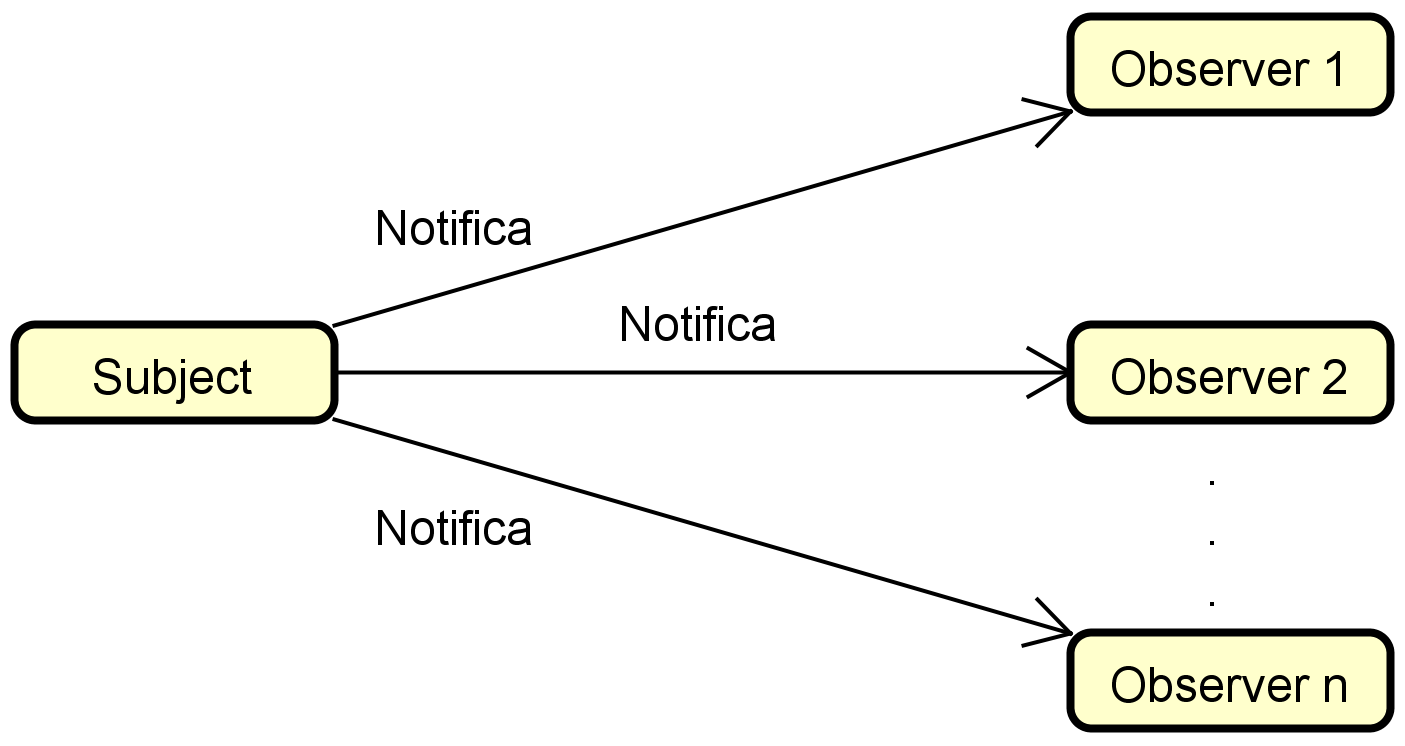
\includegraphics[scale=0.3]{Sezioni/DesignPatterns/Observer.png}
		  \caption{Schema logico del pattern Observer}
		  \end{figure}
	\item \textbf{Motivazione}: attraverso questo pattern è possibile separare le varie componenti di una applicazione web facendo sì che la parte che regola la logica dell'applicazione stessa non sappia da chi vengano emessi i vari eventi, ma sia invece in grado di recepirli e gestirli. D'altra parte, inoltre, alla parte grafica non deve interessare in seguito a che azione da parte della parte logica viene emesso un determinato evento che notifica il cambiamento di dati da mostrare, ma sia solamente in grado, utilizzando i dati trasportati con quell'evento, di aggiornarsi per mostrare tale cambiamento.
	\item \textbf{Applicabilità}: questo pattern viene utilizzato quando:
		  \begin{itemize}
		  	 	\item Si vuole poter inviare degli eventi più consistenti di quelli possibili con il pattern \termine{Event listener}.
		  	 	\item Si vuole permettere a più componenti diverse di reagire ad un determinato evento emesso da una singola componente.
		  \end{itemize}
	\item \textbf{Utilizzo}: questo pattern all'interno del progetto viene utilizzato nei seguenti casi:
		  \begin{itemize}
		  		\item Nella connessione tra l'istanza di \termine{Rocket.chat} e \progettoShort.
		  		\item Nell'interazione tra il codice HTML e la classe JavaScript associata nella sezione della \termine{View}, grazie all'utilizzo del framework \termine{Vue.js} che permette al codice \termine{Javascript} di rimanere in ascolto di eventuali interazioni da parte dell'utente con particolari oggetti HTML come i bottoni o campi di input.
		  	 	\item Nell'interazione tra \termine{View} e \termine{Presenter}, in particolare viene utilizzato per far sì che il \termine{Presenter} rimanga in ascolto (e sia pertanto l'Observer) degli eventi che si verificano all'interno della \termine{View} (che costituisce dunque il Subject) e che vengono emessi in seguito all'interazione con l'utente.
		  	 	\item Nell'interazione tra \termine{Presenter} e il database, per far sì che ogni aggiornamento che si verifica all'interno del database sia propagato correttamente anche alla parte di visualizzazione dei dati, per rendere così l'applicazione responsiva e real-time.
		  \end{itemize}
\end{itemize}

\subsection{Architetturali}
\subsubsection{Model-View-Presenter}
\begin{itemize}
	\item \textbf{Scopo}: derivato del \termine{Model-View-Controller}, questo pattern si compone di tre parti:
		  \begin{itemize}
		    	\item View: essa rappresenta la parte grafica dell'applicazione. Il suo unico scopo è inoltrare gli eventi derivati dall'interazione dell'utente con l'interfaccia grafica al Presenter, e mostrare i dati nella maniera corretta eseguendo ciò che le viene detto di fare dal Presenter. Per questo motivo essa viene definita "passiva".
		    	\item Presenter: funge da "uomo di mezzo" e serve a ricevere gli input derivanti dalla \termine{View} per eseguire di conseguenza le azioni necessarie contattando il Model. Esso inoltre rimane costantemente in ascolto del Model per eventuali cambiamenti da far visualizzare alla View.
		    	\item Model: insieme delle classi atte a modificare i dati e ad eseguire le operazioni che costituiscono la logica dell'applicazione. Esso si basa sui sistemi di persistenza dei dati come i database, e in seguito all'input derivante dai \termine{Presenter} esegue le azioni necessarie.
		  \end{itemize}	
		  \begin{figure}[H]
		  \centering
		  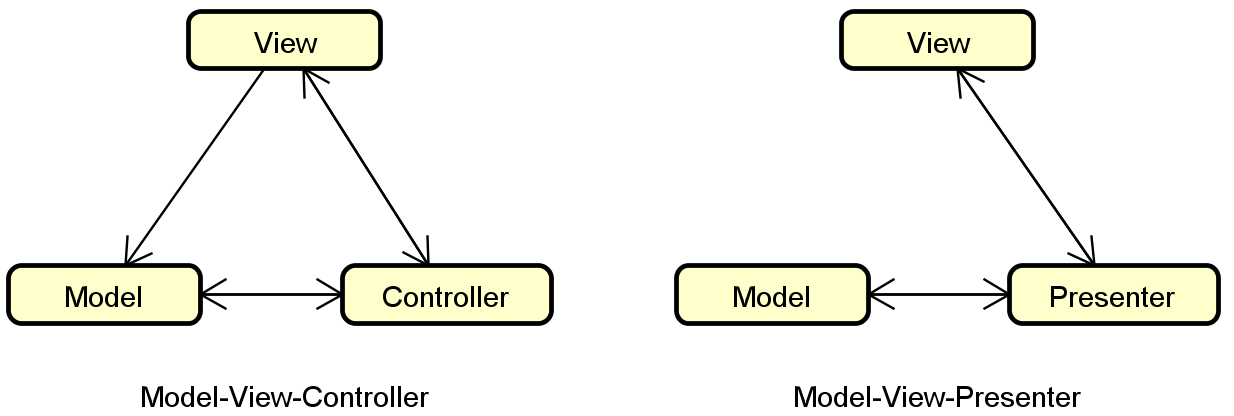
\includegraphics[scale=0.45]{Sezioni/DesignPatterns/ModelViewControllerEModelViewPresenter.png}
		  \caption{Differenza nella struttura tra pattern \termine{Model-View-Controller} e Model-View-Presenter}
		  \end{figure}	   
	\item \textbf{Motivazione}: grazie a questo pattern è possibile separare le varie componenti dell'applicazione e rendere quest'ultima più facilmente testabile. Inoltre, essendo tutte e tre le componenti indipendenti l'una dall'altra, facilita eventuali cambiamenti che potrebbero verificarsi nelle scelte architetturali durante il ciclo di vita dell'applicazione, permettendo quindi anche una maggiore manutenibilità del codice e dell'architettura stessa.
	\item \textbf{Applicabilità}: questo pattern si utilizza quando l'applicazione da realizzare possiede una componente grafica di rilevante importanza e vi è la necessità, per una migliore organizzazione, di separare le varie componenti logiche e di interfaccia grafica. Inoltre spesso viene preferita al \termine{Model-View-Controller} in quanto non vi è, come in quest'ultimo, la diretta interazione tra la parte grafica e quella logica, ma si passa invece sempre attraverso il Presenter.
	\item \textbf{Utilizzo}: all'interno di \progettoShort\ questo pattern viene utilizzato nella gestione grafica di tutte le bolle e particolari altre viste inserite all'interno dell'applicazione. Più in particolare viene adottato il seguente schema, per i widget:
\begin{itemize}
\item Le \textbf{View} saranno dei semplici template in HTML con una semplice interfaccia di comunicazione.
\item I \textbf{Presenter} verranno implementati con il design pattern comportamentale Observer, quando la View dovrà interagire con l'utente e di conseguenza il Presenter deve poter ricevere questi aggiornamenti. Se, invece, la View non deve essere aggiornata poiché statica, non verrà utilizzato il Pattern Observer, ma l'interazione sarà mantenuta solo per rimanere coerenti al Pattern e permettere una futura implementazione interattiva per chi volesse un giorno espandere l'\termine{SDK}.
\item I \textbf{Model} per i widget non saranno disponibili nell'\termine{SDK}, questo perché dovrà essere lo sviluppatore a definire il loro  comportamento, ovvero la loro \termine{Business-Logic}, mantenendo così la struttura del pattern.
\end{itemize}
Lo schema Model-View-Presenter verrà utilizzato anche nell'applicazione \app\ per ogni azione o componente.
Essendo totalmente definita e non ampliabile dallo sviluppatore (come per l'\termine{SDK}), l'applicazione definirà, oltre alla View e al Presenter, anche il Model. Quest'ultimi verranno caricati nella parte Server del programma seguendo la suddivisione logica dei programmi \textit{Meteor}.
\end{itemize}

\subsubsection{Clean Architecture}
\begin{itemize}
	\item \textbf{Scopo}: pattern simile al \termine{Model-View-Presenter} e ideato da Robert Cecil Martin, questo pattern scompone in maniera ancora più approfondita le componenti di una applicazione dividendole in quattro parti una interna all'altra, dal più esterno al più interno:
	\begin{itemize}
	  	\item Strato \textbf{esterno}: contiene i database, l'interfaccia grafica e tutte le altre componenti come framework e drivers.
	  	\item Strato \textbf{intermedio esterno}: contiene tutte quelle interfacce che permettono allo strato esterno di comunicare con quello intermedio interno. Oltre ad esse sono anche presenti le varie classi che permettono di convertire i dati dai formati utilizzati nello strato esterno a quelli utilizzati nello strato intermedio interno e viceversa.
	  	\item Strato \textbf{intermedio interno}: contiene gli \textit{use case}, ovvero quelle classi che compongono le regole logiche dell'applicazione e rappresentano il corrispettivo del Model nel modello Model \termine{View} Presenter.
	  	\item Strato \textbf{interno}: contiene tutte quelle classi che rappresentano gli oggetti che descrivono le regole logiche dell'intera azienda. Visto il loro utilizzo molto specifico, esse non verranno utilizzate nel nostro caso, di fatto rendendo questo strato per noi vuoto.
	\end{itemize}
	\begin{figure}[H]
	\centering
	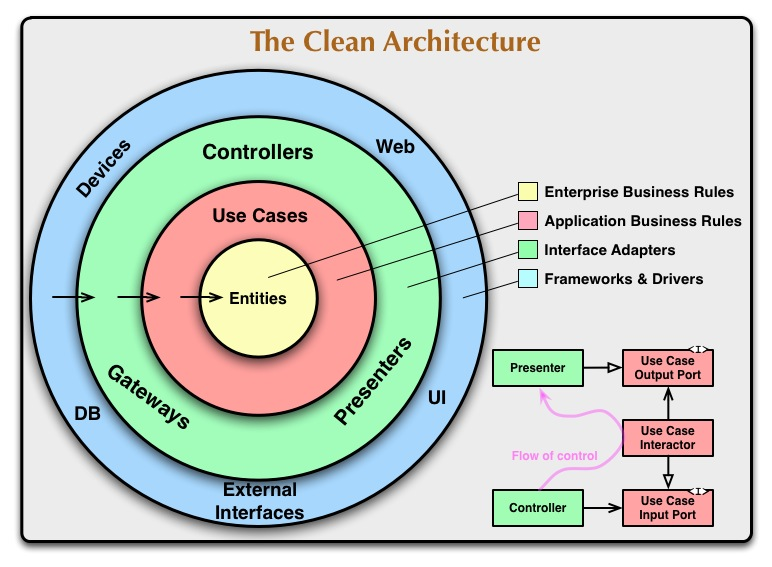
\includegraphics[scale=0.3]{Sezioni/DesignPatterns/CleanArchitecture.jpg}
	\caption{Schema a strati del pattern architetturale Clean Architecture}
	\end{figure}
	
	Oltre a questo, all'interno di questa architettura vige la \textit{dependency rule}, secondo la quale le dipendenze possono essere solamente orientate verso l'interno e di conseguenza gli strati più interni non posso dipendere da quelli più esterni. Per poter rispettare questo vincolo spesso viene utilizzato il \termine{dependency inversion principle} assieme al metodo dell'\termine{Inversion of Control} mediante \termine{dependency injection}.
	\item \textbf{Motivazione}: grazie a questo pattern è possibile dividere ulteriormente le varie componenti dell'applicazione, rendendola di conseguenza maggiormente testabile e mantenibile. Oltre a ciò, grazie ai vari adapter posti tra uno strato e l'altro, essa permette di rendere i vari strati esterni indifferenti ad eventuali cambiamenti negli strati più interni e viceversa.
	\item \textbf{Applicabilità}: questo design pattern viene utilizzato quando si vuole creare una applicazione che sia, in ogni suo componente, facilmente modificabile senza dover andare a riscrivere grandi quantità di codice. Esso viene particolarmente in aiuto nello sviluppo di applicazioni che utilizzano vari framework, librerie e componenti di terze parti propense a cambiare nel tempo e che devono poter rispondere a tali cambiamenti in maniera rapida ed efficace.
	\item \textbf{Utilizzo}: questo design pattern viene utilizzato nello sviluppo dell'applicazione demo, in particolare nella gestione delle bolle e della logica ad esse connesse, oltre che alla creazione dell'interfaccia grafica e della logica di eventuali altre viste in essa presenti. E' stato scelto questo tipo di architettura poiché funziona molto bene con il pattern MVP e poiché suddivide bene gli strati, i loro ingressi e le loro uscite. Inoltre come riferito nel \textit{Verbale interno} del 26 Febbraio 2017 ed in particolare nella decisione \textit{VI4.3}, gli strati sono i seguenti:
\begin{itemize}
\item Il primo è lo strato più esterno e gestisce la comunicazione con tutto ciò che non è interno all'applicazione.
\item Il secondo fa riferimento ai vari presenter che fanno da tramite tra il Model e la View.
\item Il terzo fa riferimento alla \termine{Business Logic}, ovvero ai model.
\item Il quarto rappresenta il database.
\end{itemize}
\end{itemize}
 